\documentclass[thesis.tex]{subfiles}
\begin{document}
\chapter{Future Work}

Throughout this thesis we have described the policies of the mobile
ecosystem and how AppPAL can be used to describe them.  We have argued
that AppPAL is a good language for describing these policies, however
there are also areas where AppPAL could be improved to further to
describe more kinds of policies and to aid policy authors.  This
chapter looks at two areas in particular and describes our
\emph{preliminary} explorations.  We describe how AppPAL policies can
be analyzed automatically and describe an early prototype to check
policies for common problems.  We also describe preliminary thoughts
about how plausibility, quantified doubt, could be used to express
confidence in a statement.

\section{Automatic Analysis of AppPAL policies}
\label{sec:lint}

When examining an AppPAL policy it is natural to wonder whether the
policy is as optimal, in terms of the rules and facts required to
decide a query and the number of rules in the policy, as it could
be. Is a decision reachable given the rules and facts contained in the
policy?  Does an assertion context contain enough statements to use a
given rule? If there are multiple ways of deciding whether some
statement is true or not does one rule require fewer statements than
any other? Does one rule require only a subset of the facts of another
rule, implying the second is redundant?

Many authorization and logic-programming languages, such as
XACML~\cite{ramli_detecting_2015} and
Datalog~\cite{alon_levy_equivalence_1993,alon_levy_constraints_1992}, have
thought about how policies can be checked for various properties
similar to those described here.  The properties we seek to check
AppPAL (or SecPAL) for are not novel, but rather the application of
them to SecPAL is.

We have implemented preliminary checkers for some of these properties,
though they are undertested.  The code is included with AppPAL.

\subsection{Checking Satisfiability}

If an assertion is \emph{satisfiable} then there are sufficient facts
such that the assertion's conditions could be met.  We care about this
property when writing policies as it means that our assertions affect
something.  If an assertion is \emph{unsatisfiable} then this may
indicate that we have failed to specify one of the conditions it
depends upon.

When an assertion is satisfiable there is a combination of facts that
could satisfy its conditionals. If there are no facts that could
satisfy the rule then the policy may be unsatisfiable as there are
rules that can never be used.  For any goal $G$:

\begin{align*}
  G \in \text{Satisfiable}~\text{\textit{if}}~\exists A \in \text{AC}:~&\exists \theta:~G\equiv\text{head}(A\theta) \\
                                                              \wedge~ & (\text{conditionals}(A) = \emptyset \\
                                                                      & \vee~\forall G^\prime \in \text{conditionals}(A).~G^\prime \in \text{Satisfiable}.)
\end{align*}

This is a similar idea to the notions of \emph{satisfiability} in Datalog (and
more generally logic programming).  Satisfiability in Datalog is defined
as~\cite{alon_levy_equivalence_1993}:

\begin{quote}
  \textbf{Satisfiability:} An IDB predicate $s$ of a program $P$ is
  \emph{satisfiable} if there is some EDB $D$, such that $P$ defines a
  non-empty relationship for $s$.
\end{quote}

For an example of satisfiability, consider the following snippet taken
from the NHS policy described in \autoref{chap:byod}.  The rule
described in the policy is that an app must be approved by the
\ac{IGC} as well as by either the \ac{CACPG} as well as the \ac{MIG}
depending on whether it is for clinical or business use. We describe
this in AppPAL as:

\begin{lstlisting}
'nhs-trust' says App isInstallable
  if App isApproved, App isUsableClinically.
'nhs-trust' says App isInstallable
  if App isApproved, App isUsableNonClinically.
'nhs-trust' says 'igc' can-say App:isApproved.
'nhs-trust' says 'cacpg' can-say App:A isUsableClinically.
'nhs-trust' says 'mig' can-say App:A isUsableNonClinically.
\end{lstlisting}

What apps in practice are approved for use?
As the policy document notes, none of the groups or committees have ever
approved an app in practice.
When we run the satisfiability checker on this policy
it reports that (amongst other information) no app is installable.

\begin{lstlisting}
$\$$ java -jar Lint.jar --satisfiability example.policy
[INFO]: loaded 1/1 files of 6 assertions
Issues identified when checking satisfiability.
The following decisions may be unsatisfiable by their speakers:
'nhs-trust' says * isUsableClinically
'nhs-trust' says * isInstallable
'nhs-trust' says * isApproved
'nhs-trust' says * isUsableNonClinically

In particular the following assertions are unsatisfiable:
'nhs-trust' says App isInstallable if App isApproved, App isUsableNonClinically.
'nhs-trust' says App isInstallable if App isApproved, App isUsableClinically.

These decisions may be satisfiable through delegation but we
lack any statements to that effect from the delegated party:
(via 'cacpg') 'nhs-trust' says * isUsableClinically
(via 'igc') 'nhs-trust' says * isApproved
(via 'mig') 'nhs-trust' says * isUsableNonClinically
\end{lstlisting}

As well as reporting which decisions it cannot make, it also reports the
specific assertions as well.

Using AppPAL we can describe policies using delegation. As well as looking for assertions that are unsatisfiable it also looks for examples where we have a \emph{can-say} statement, but lack any statements from the delegated party to that effect.  This may indicate that we need to collect additional statements from the delegated person, or that the \emph{can-say} statement can be removed as it will not be used.
This check is somewhat simple and we don't take into account dependencies
between variables.  If we add, for example, the statements:

\begin{lstlisting}
'igc' says 'angry-birds' isApproved.
'cacpg' says 'dropbox' isUsableClinically.
'mig' says 'instagram' isUsableNonClinically.
\end{lstlisting}

Then we will still never find any installable apps, as the \ac{IGC},
\ac{CACPG} and \ac{MIG} need to agree on the same app to find it
installable.  When we run the satisfiability checker however, we find
no problems as all the decisions are now satisfiable as there is a
decision about \emph{some} variable; even if that variable isn't
useful in practice.

\begin{lstlisting}
$\$$ java -jar Lint.jar --satisfiability example.policy
[I]: loaded 1/1 files of 11 assertions
[I]: no satisfiability problems
\end{lstlisting}

The satisfiability checker acts as a quick sanity checker that a policy contains
enough facts and assertions. unlike AppPAL-proper which can check how and whether a specific statement would be be made.

%The code in \autoref{alg:reachable} produces a set of pairs of predicates and
%speakers where the pair of a speaker and a predicate indicates that that
%speaker may say something about that predicate. We search over all the
%assertions in the AppPAL assertion context. If all of an assertion's
%conditionals (the facts in the if part) are reachable (or it has none) then the
%speaker and predicate are added to the reachable set. If the statement is a
%can-say statement then we additionally check if the delegated predicate is
%reachable from the delegated speaker, and if so mark the delegated statement as
%reachable from the speaker who made the can-say statement.
%
%\begin{lstlisting}[language=Python,float,caption={Procedure for finding all reachable assertions.},label={alg:reachable}]
%def reachable(ac) -> set:
%  reachable = new set()
%  iterate = True
%  while iterate == True:
%    iterate = False
%    for assertion in ac:
%      e = a.speaker
%      p = a.predicate
%      if p.isCanSay() and (e, p) in reachable:
%        if (p.delegator, p.delegation) in reachable:
%          if for all c in a.conditions: (e, c.predicate) in reachable:
%            reachable.add((e, p.delegation))
%            iterate = True
%      else if not (e, p) in reachable:
%        if for all c in a.conditions; (e, c.predicate) in reachable:
%          reachable.add((e, p))
%          iterate = True
%  return reachable
%\end{lstlisting}

\subsection{Checking Redundancy}

If unsatisfiability can be caused when we lack sufficient facts and assertions to make a decision then redundancy occurs when we have too many.  Specifically there are two types of redundancy~\cite{alon_levy_constraints_1992} that we care about here:

\begin{itemize}
\item \emph{Unreachability} occurs if a predicate does not take part in the
  minimal deverivation tree of a fact.
\item \emph{Irrelevance} occurs if a derivation tree contains pairs of identical atoms.
\end{itemize}

These ideas are directly relatable to AppPAL, for instance if we have the
following AppPAL policy:

\begin{lstlisting}
'alice' says App isInstallable
  if App isRecommended,
     App isNotMalware.

'alice' says App isRecommended
  if App isNotMalware,
     App isGood.
\end{lstlisting}

Alice checks that the app is not malware when checking the app is
installable and when checking that the app is recommended.  The check
in \texttt{isInstallable} is irrelevant as it depends on the app being
recommended which also checks this property.  When writing AppPAL
policies this kind of irrelevance commonly occurs when using the
typed-syntax described in \autoref{ssec:types}. For example, in this
excerpt from a SANS BYOD policy there is a check that \emph{U} is a
user in both assertions.  In the first there is irrelevance because
\emph{U} is stated as being a user twice, where once would have been
sufficient.  In the second there is a single check that \emph{U} is a
user but it is irrelevant as the check had already been done when
checking is \emph{U} had lost the device (since only users can lose
devices in the first assertion).

\begin{lstlisting}
'company' says User:U can-say User:U hasLost(Device:D)
  if D isOwnedBy(U).

'company' says User:U mustInform('help-desk', 'device-lost')
  if U hasLost(Device).
\end{lstlisting}

We can check for this kind of irrelevance by building a proof-graph for the
assertion context.  Every node (shown in a box) represents an AppPAL fact we
might wish to prove.  For every assertion in the context we create a proof
(represented as a number in brackets) for the head of the assertion, which is
connected to the facts required to prove the assertion.  In the case of can-say
and can-act-as statements we expand them as per AppPAL's inference rules.
A proof-graph for the above example is shown in \autoref{fig:irrelevance}: the
irrelevant links are shown in red and the AppPAL facts connected to the two
dashed ones can be removed to remove the irrelevance.

\begin{figure}
  \centering
  \includegraphics[width=0.5\linewidth]{./figures/irrelevance.png}
  \caption{Proof graph showing irrelevance.}
  \label{fig:irrelevance}
\end{figure}

In contrast unreachability occurs when a fact does not take part in the minimal
derivation tree of a fact.  As a simple example consider the following policy:

\begin{lstlisting}
'alice' says App isInstallable if App isNotMalware.
'alice' says App isInstallable if App isNotMalware,  App isRecommended.
\end{lstlisting}

To detect unreachability for a given policy we again build the proof-graph (shown
in \autoref{fig:unreachability}).  For each proof node we collect the facts
(the leaves of the graph underneath it, which are the ground assertions from the
AC\footnote{Or in the case of an unsatisfiable policy facts with variables that
  cannot be unified with a ground fact.} in
AppPAL).  If the facts for one proof node connected to a fact are a subset of
the facts for another proof node, then the larger proof node, is unreachable it
contains facts which are not in the minimal derivation tree.   In the case of
\autoref{fig:unreachability}, the derivation-graph 2 is made redundant by
derivation-graph 1 as it contains a subset of the facts.  This is a
simplified example; in general facts lower in the tree may have multiple
derivation trees, leading to multiple sets of facts being required for a fact
that seems to have only one proof node.  Loops can also occur (where one fact
depends on itself to prove itself).  This approach isn't complete, but it does
identify several cases where an AppPAL policy may be redundant through
unreachability.

\begin{lstlisting}[float, caption={Output of AppPAL when checking a policy with unreachability.}]
java -jar Lint.jar --redundancy unreachable.policy
[I]: loaded 1/1 files of 2 assertions
[I]: flattened 0 node(s)
[W]: 'alice' says App isInstallable. has unreachable derivation trees.
\end{lstlisting}

\begin{figure}
  \centering
  \includegraphics[width=0.5\linewidth]{./figures/unreachability.png}
  \caption{Proof graph showing unreachability.}
  \label{fig:unreachability}
\end{figure}

Redundancy can occur when there are multiple rules that result in the
same decision being made.  Rules may depend on other rules, or ground
facts.  One proof ($A$) is made redundant by another proof ($B$) if
the set of ground facts used in $B$ is a subset of the ground facts
used in $A$. Whenever $A$ is satisfied $B$ will also be, but when $B$
is satisfied $A$ may not be: consequently $A$ is redundant as $B$ can
be used to prove its goal with fewer facts.  For any goal
$G$.

\begin{align*}
  \exists p_1 \in \text{proofs}(G).~\exists p_2 \in \text{proofs}(G).        & \\
  p_1 \not= p_2~\wedge~\text{facts}(p_1) \subset \text{facts}(p_2)           & \implies G\text{ has unreachable proofs.} \\
  p_1 \not= p_2~\wedge~\text{facts}(p_1) = \text{facts}(p_2)                 & \implies G\text{ has equivalent proofs.}
\end{align*}

Additionally if two different goals ($G$ and $G^\prime$) have
equivalent proofs, then we report this as it implies the two
statements may not be independent.

\begin{align*}
  \exists p_1 \in \text{proofs}(G).~\exists p_2 \in \text{proofs}(G^\prime). & \\
  \text{facts}(p_1) = \text{facts}(p_2)                                      & \implies \text{$G$ and $G^\prime$ have equivalent proofs.}
\end{align*}

A simple example might be the policy shown in \autoref{fig:redundancy-graph-simple}.
The second rule makes the first redundant.  We can represent the policy
as a graph shown opposite the policy.  The goal (shown as a blue rectangle) has two routes
to prove it true (each shown in ellipses).  Route 1 requires that the facts
(shown in green rectangles) \lstinline!'x' says 'y' r,! and
\lstinline!'x' says 'y' q.!, whereas route 0 only requires the
latter fact.

\begin{figure}
  \centering
  \begin{minipage}{0.4\linewidth}
    \begin{lstlisting}
'x' says 'y' p
  if 'y' q,
     'y' r.

'x' says 'y' p
  if 'y' q.
    \end{lstlisting}
  \end{minipage}
  \begin{minipage}{0.59\linewidth}
    \scriptsize{}\centering
    \def\svgwidth{\columnwidth}
    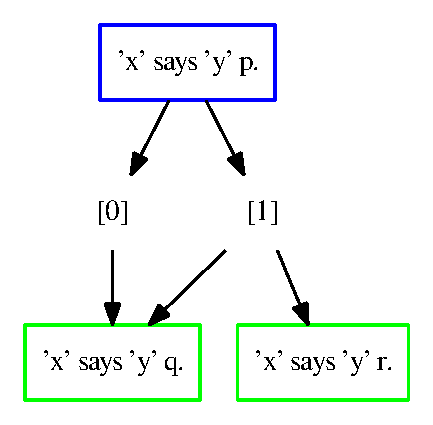
\includegraphics[width=0.59\linewidth]{figures/redundancy-simple.eps}
  \end{minipage}
  \caption{A simple policy shown as a graph.}
  \label{fig:redundancy-graph-simple}
\end{figure}

A more complex example is shown below:

\begin{lstlisting}
'x' says 'z' p if 'z' q.
'x' says 'y' can-say 'z' p.
'y' says 'z' p if 'z' q.
'y' says 'x' can-say 'z' q.
\end{lstlisting}

Representing this policy as the graph in \autoref{fig:redundancy-complex} we can see it is more complex. Goals that
depend on more than just green facts, are shown as black rectangles.  If a goal
is used to prove another goal, and it itself only depends on green, ground,
facts, then the node is marked to be flattened (red rectangle).  Its proofs are
merged into the higher proof, and the flattened goal is removed from the higher
proof.  This process is repeated until no more nodes can be flattened (shown
twice in \autoref{fig:redundancy-complex}).  Once the graph is flattened we can
identify that \lstinline!'x' says 'z' p! has a redundant means of proof (route
0 only uses one of route 1's facts).  We can also see that all the proofs for
\lstinline!'y' says 'z' q! and \lstinline!'y' says 'z' p! use the same facts.
We report these statements as having equivalent proofs as the goals are not
independent of each other (implying we could use fewer goals and still write
equivalent policies).

\begin{figure}
  \centering\tiny
  \framebox{\def\svgwidth{0.35\linewidth}1.
    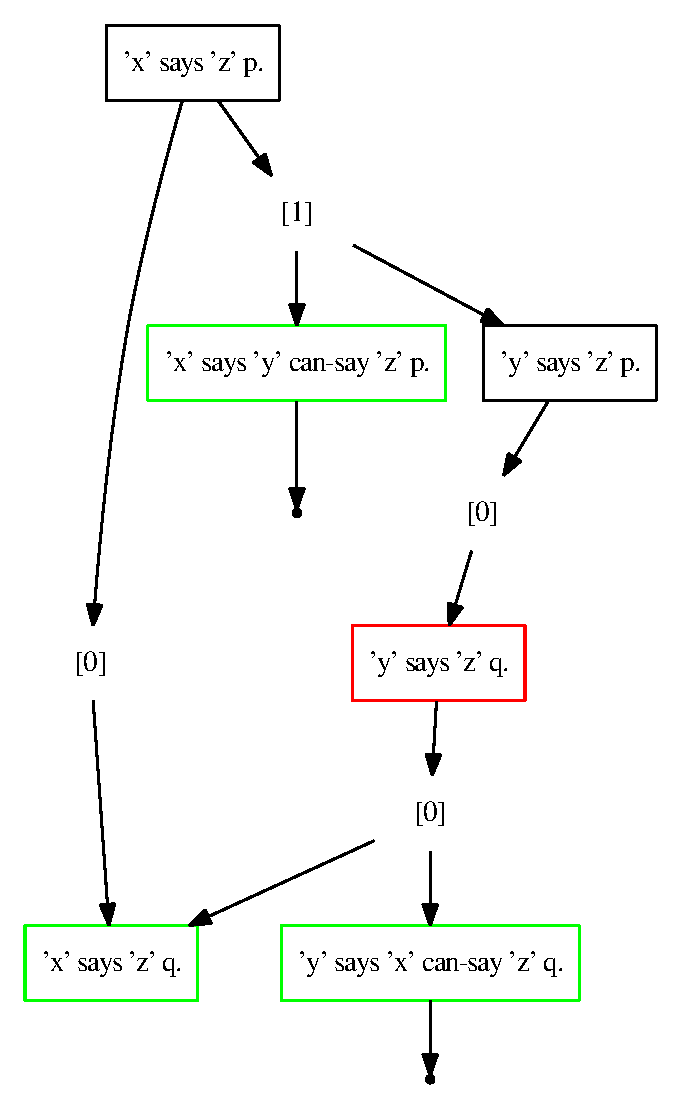
\includegraphics[width=0.35\linewidth]{figures/redundancy-complex-0.eps}}
  \framebox{\def\svgwidth{0.55\linewidth}2.
    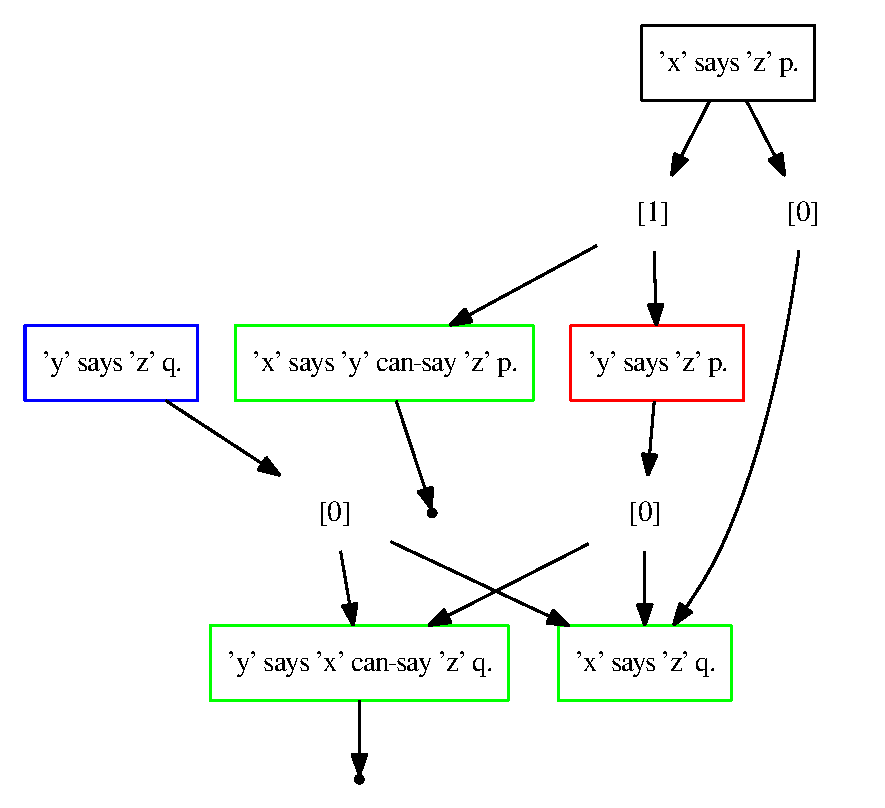
\includegraphics[width=0.55\linewidth]{figures/redundancy-complex-1.eps}}
  \newline
  \framebox{\def\svgwidth{0.8\linewidth}3.
    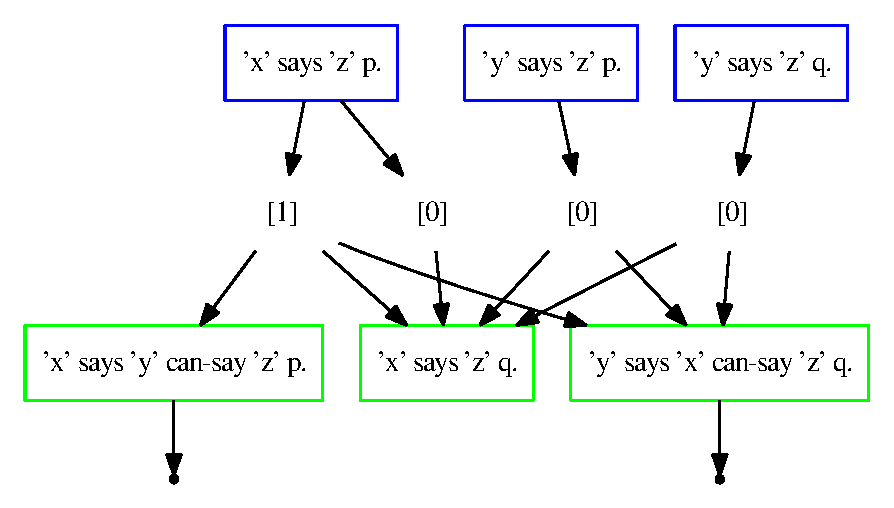
\includegraphics[width=0.8\linewidth]{figures/redundancy-complex-2.eps}}
  \caption{Flattening a more complex policy.}
  \label{fig:redundancy-complex}
\end{figure}

% To build the graphs, each statement we might want to prove (a goal) becomes a
% node in the graph, its children are organised into sets of goals (a proof),
% where if all the goals in any set were proved true then the goal node would also
% become true. If a node has an empty set of goals to prove it is a fact. Once the
% graph has been constructed (taking into account delegation and unification with
% other statements), the graph is flattened by applying the flatten procedure
% (Listing~\ref{alg:flatten}) repeatedly until a fixed point is reached. When the
% graph has been flattened we look for redundancy by looking for goals with proofs
% that are subsets of their other proofs, implying that if the larger proof is
% true, then the shorter proof will always be true too; and different goals with
% identical proofs, implying that the two decisions are not
% independent~(Listing~\ref{alg:redundancy}).

% \begin{lstlisting}[language=Python,float,caption={Procedure for flattening the redundancy graph.},label={alg:flatten}]
% def flatten(graph):
%   for goal in graph.goals:
%     hoist = true
%     for proof in graph[goal]:
%       for proof_goal in proof:
%         if not proof_goal.is_fact:
%           hoist = False
%           break
%       if hoist == True:
%         hoist(graph, goal)

% def hoist(graph, target):
%   for parent in graph[target].parents:
%     for proof in parent.proofs:
%       if proof.uses(target):
%         for replacements in graph[target].parents:
%           parent.proofs += proof.replace(target, replacements)
%           parent.proofs -= proof
% \end{lstlisting}

% \begin{lstlisting}[language=Python,float,caption={Procedure to check for redundancy.},label={alg:redundancy}]
% def check_redundancy(graph) -> boolean:
%   for goal in graph.goals:
%     for a in graph[goal]:
%       for b in graph[goal]:
%         if a >= b and a.goals.subset(b.goals):
%           if b.goals.subset(a.goals):
%             warn(a+" has multiple equivalent proofs")
%           else
%             warn(a+" has a redundant proof")
%     for other_goal in graph.goals:
%       if goal > other_goal:
%         for a in graph[goal]:
%           for b in graph[other_goal]:
%             if not (a.goals.is_empty() or b.is_empty())
%                and a.goals == b.goals:
%               warn(a+" and "+b+" have equivalent proofs")
% \end{lstlisting}

\section{Plausible AppPAL}

\newcommand{\secpalmath}[1]{\ensuremath\texttt{#1}}
\newcommand{\AC}[0]{\ensuremath\text{AC}}
\newcommand{\says}[1]{\ensuremath~\secpalmath{says}^{\new{#1}}~}
\newcommand{\canSay}[1]{\secpalmath{can-say}_{#1}}
\newcommand{\canActAs}[0]{\secpalmath{can-act-as}}
\newcommand{\spif}[0]{\secpalmath{if}}
\newcommand{\where}[0]{\secpalmath{where}}

The SecPAL authorization language, and the AppPAL instantiation, allow
policy authors to make use of static analysis tools to make decisions,
and allow principals to make statements about apps through delegation.
When these decisions are made they are made with certainty.  If a
principal says an app is safe to access the network then we believe
that that principal definitely believes the app is safe on a network.
When a static analysis tool finds that an app isn't malware then we
believe that app to not be malware.  This isn't realistic.  Static
analysis tools can produce false results.  A principal might be merely
fairly confident that an app can access the network but not absolutely
certain.

With current authorization languages, such as AppPAL and XACML, there
is no way to quantify the belief a principal has in any statement.  A
principal cannot say how plausable they think any statement is.

\subsection{Examples of Plausability}

SecPAL was designed to make access control decisions.  The decision
whether to install allow a user access to a file or not is a binary
one: either they can access it or they cannot.  Similarly the decision
process for these decisions is also binary: a user is either logged in
or not, a network address is either in the network or outside it,
someone can act as someone else's manager or they can not.

AppPAL, however, is primarily for deciding what apps you want to use.
Whether you want to install an app or not is less binary than an
access control decision, because it is ultimately an opinion.
Consider a really simple policy that says \emph{``do not install
malware''}: you could try using a malware scanner to check apps, but
there opinions on apps can change rapidly and often.  You could use a
meta-scanning tool like \emph{VirusTotal}, but then you'd only get the
percentage of antivirus tools that flagged the app as
malicious~(\autoref{fig:android-malware}).  The scan in
\autoref{fig:android-malware} was for a sample of the
\emph{BaseBridge} malware, taken from the \emph{Android Malware Genome
Project}~\cite{zhou_dissecting_2012}.  Even for this relatively old
malware sample (from 2012) 15 antivirus programs, including McAfee and
Yandex's programs, did not flag it as dangerous.  In contrast a scan
of the \emph{towelroot}
app~\cite{george_geohot_hotz_towelroot_nodate}, an app which will
grant root access to a device but is not \emph{in itself} malicious, 3
out of 64 antivirus checkers reported the download source as
dangerous.  If the app were to be installed on a device then a further
warning would be displayed by Google's own built-in antivirus.  This
last app is not technically malicious, but it is certainly dangerous.
The assertion that an \emph{app is safe} is not a binary decision.
Without plausability we cannot represent the doubt and confidence in
any assertion.

\begin{figure}
  \centering
  \includegraphics[width=\linewidth]{figures/android-malware.png}
  \includegraphics[width=\linewidth]{figures/towelroot.png}
  \caption[VirusTotal results for two Android apps.]{VirusTotal results for 57 antivirus packages scanning a sample of the BaseBridge Android malware, and 64 antivirus packages analyzing a download of the Towelroot rootkit.}
  \label{fig:android-malware}
\end{figure}

For another example consider a policy you only want to install apps
that are made by \emph{reputable} developers and that are \emph{safe}.
Both reputable and safe are poorly defined, and badly represented by a
binary decision.  A developer may be reputable if they are a large
developer with a lot of staff like Google or Facebook, they might be
reputable if their apps have been well reviewed, but what about a
developer who produces a large number of games with
in-app-purchases, TV adverts, and sketchy privacy records.  They are
probably more reputable than a malware author but you might have less
confidence that they are producing good apps than Google.
An app might be seen as safe if it doesn't request any permissions and
has no native code, but if it starts requesting more permissions and
the amount of native code grows then a user's confidence that it is safe
might fall.  When combined into the policy as a whole Google may be
able to get away with a lot more permissions than other developers
simply because users trust them more not to be evil.  Again, without
plausability it is difficult to represent these decisions.

Probabilistic versions of Datalog are not a new idea.  Various papers proposed
probabilistic variants of Datalog~\cite{fuhr_probabilistic_1995} or explored the
semantics of probabilistic logics~\cite{halpern_analysis_1990}.  Role-based
access control languages have incorporated ideas about risk into their
schemes~\cite{josang_analysing_2004,dimmock_using_2004,salim_approach_2011},
which is a similar notion to plausability and trust.  These schemes do not seem
to deal with delegation in the same manner as SecPAL however so incorporating
similar ideas here may be interesting and allow SecPAL and AppPAL greater
expressiveness.  Part of the work toward this this year has included modifying Becker's
evaluation and translation-to-Datalog algorithms~\cite{becker_secpal:_2010} to
include a plausability value, and for giving rules to query on the basis of
them, using Datalog$^C$~\cite{li_datalog_2003}.

\subsection{Modifying AppPAL for Plausability}

AppPAL has three rules for evaluation: \emph{cond}, \emph{can-say},
and \emph{can-act-as}.  We modify the language so that the \emph{says}
keyword has an an annotation $0 \geq p \geq 1$ denoting a statements
\emph{plausability}.  If the annotation is missing then it is assumed
to be $1$ We also assume a plausability combining function $\oplus$
which combines plausability.  The AppPAL inference rules then become
as follows, with additions highlighted in \new{red}.

{\footnotesize\centering
\begin{equation*}
  \infer[\text{cond\new{$\leq$}}]{
    \AC{}, D \models A~\says{\bigoplus_{i=1}^n p_i}~f\theta
  }{
    \begin{matrix}{
      \left(A~\says{}~f~if~f_1\cdots f_n~\where~c~\new{\text{with plausability at least}~p_{lim}}\right) \in \AC{}
    }\\{
      \forall i \in [1\cdots n]. \AC{}, D \models A~\says{p_i}~f_i\theta
    }\\\new{
      0 < p_{lim} \leq \bigoplus_{i=1}^n p_i
    }
    \end{matrix}&
    \vdash c\theta &
    vars\left(f\theta\right) = \emptyset
  }
\end{equation*}
\begin{equation*}
  \infer[\text{cond\new{=}}]{
    \AC{}, D \models A~\says{p_{lim}}~f\theta
  }{
    \begin{matrix}{
      \left(A~\says{}~f~if~f_1\cdots f_n~\where~c~\new{\text{with plausibility is}~p_{lim}}\right) \in \AC{}
    }\\{
      \forall i \in [1\cdots n]. \AC{}, D \models A~\says{p_i}~f_i\theta
    }\\\new{
      0 < p_{lim} \leq \bigoplus_{i=1}^n p_i
    }
    \end{matrix}&
    \vdash c\theta &
    vars\left(f\theta\right) = \emptyset
  }
\end{equation*}
\begin{equation*}
  \infer[\text{can-say}]{
    \AC{}, \infty \models A~\says{p_1 \oplus p_2}~f
  }{
    \AC{}, \infty \models A~\says{p_1}~B~\canSay{D}~f &
    \AC{}, D \models B~\says{p_2}~f
  }
\end{equation*}
\begin{equation*}
  \infer[\text{can-act-as}]{
    \AC{}, D \models A~\says{p_1 \oplus p_2}~x~vp
  }{
    \AC{}, D \models A~\says{p_1}~x~\canActAs~y &
    \AC{}, D \models B~\says{p_2}~y~vp
  }
\end{equation*}
\begin{equation*}
  \new{
    \infer[\text{reduce}]{
        \AC{}, D \models A~\says{p}~f
    }{
        \AC{}, D \models A~\says{p^\prime}~f & p \leq p^\prime
    }
  }
\end{equation*}
}

In general any derived statement is at most as plausible as the
combination of the statements that went into deriving it.  We split
the \emph{cond} rule into two variants.  The \emph{cond$\leq$} rule
allows us to specify a minimum plausability required by combining all
the conditional statements and if that limit is exceeded we take the
combined probability in the plausability of the outcome.  The
\emph{cond=} rule allows us again to set a minimum plausability but
this time we take the stated plausability if the rule is satisfied.
These two \emph{cond} rules serve different purposes.  The
\emph{cond=} variant is useful when we want to set a limit on the
plausability: for instance when we have a tool with a known confidence
rate we want to run, or a fact which we know how plausible it is.  The
\emph{cond=} rule is useful for when you want to ensure that a
decision is made with a certain least-confidence, for instance if you
want to be at least 80\% sure that an app is safe to use before doing
anything with it.  In this case we would want the combined
plausability to trickle through the proof not the lower limit.

We also add a plausability reduction rule that allows us to reduce the
plausability of an assertion, this allows us to phrase a policy query
as \emph{``is it at least 50\% plausable that...''} rather than having
to discover the plausabilities precisely.

\subsubsection{Plausability Combination}

How should the plausability combination operator be defined?  One
simplistic approach might be to take the least plauable assertion as
the final value.  This however is too simple. Consider the case where
an app needs to be safe and from a reputable developer.  Say we're
50\% sure the app is safe but we are unsure of the developer. We are
90\% sure Google is reputable and only 60\% sure Rovio is.  No matter
who the developer is the combined probability is the same (50\%) so
the distinction is lost.

\begin{equation*}
  p_a~\oplus_{\text{min}}~p_b~\gets~\text{min}~p_a~p_b
\end{equation*}

If we are sure the plausabilities are independent we could multiply
them together to get the final plausability. This is appealing in that
if we take the example above if Google is the developer we're 45\%
sure the app is usable, but only 30\% if Rovio is.  If however there
are a lot of combinations to be made the probabilities may get very
small and be difficult to distinguish.

\begin{equation*}
  p_a~\oplus_{\text{ind}}~p_b~\gets~p_a\times p_b
\end{equation*}

Both the two previous suggestions are na\"ive in their approach.  The
first is unnecessarily conservative, the second assumes independence.
A better scheme may be to incorporate a more sophisticated reasoning
system.  One system might be Dempster-Schafer
theory~\cite{dempster_upper_1967,glenn_shafer_mathematical_1976} which
is designed to reason about the probability of provability of any
statement. It can also be used to give a value to how close evidence
comes to rendering a proposition
provable~\cite{pearl_probabilistic_2014}. Other schemes, and working
out how to implement and integrate this into AppPAL is left to future work.

\subsection{Guarantees for Plausible AppPAL} 

However plausibility combination is implemented some thought should be
given to what properties and guarantees AppPAL ought to offer.  One
guarantee might be that if all statements are perfectly plausible then
this ought to be equivalent to standard AppPAL.  Another might be that
if a statement is perfectly implausible then it ought to be equivalent
to the statement not existing at all. A third rule should be that we
can't make a statement more plausible by combining less plausible
statements.  To summarize:

\begin{itemize}
\item If all statements have a plausability of $1$, then this is
  equivalent to standard AppPAL.
\item If a statement has a plausability of $0$, then it is equivalent
  to the statement not existing in the assertion context.
\item No statement should be more certain than the conditionals used
  to derive it.
\end{itemize}

Point 1 is true since if $p_{\text{lim}} = 1$ then no statement will
be accepted unless its plausability is also 1.  If we combine the
plausability of two events this will also be 1 (using either method
described so far): hence the restriction on the plausability in the
cond rule is always true since all statements have a plausability of
one.  Rewriting the rules with this in mind we get the original AppPAL
inference rules, so if all statements have a plausability of 1, then
this must be equivalent to standard AppPAL.

Point 2 is also true by the restriction on probabilities in the cond
rule.  Since $p_{\text{lim}}$ must be greater than 0, if a statement
has a plausability of 0 then it will not be accepted.  Similarly when
combining plausabilities if a statement is completely inplausible then
the plausibility of it happening with another event must also be
implausible.  Hence the combination should always be 0, and no
statement combined with an implausible statement will be derivable.

Point 3 is important as we don't want a means to make a statement more
certain by repeatedly applying a rule.  For example imagine we had a
combination operator that took the sum (or 1 if the combination was
greater than 1), and a rule such as:

\begin{lstlisting} 
'x' says 'y' p if 'y' p, 'y' p.
\end{lstlisting}

If we also have statement that $x \says{0.2} y p$,
then we could apply this rule to get $x \says{0.4} y p$, and so on
until we're certain.

Similarly if we had statements  such as:
\begin{lstlisting} 
'x' says 'y' p 
  if 'y' p,
     'z' p.
\end{lstlisting}

If we knew, with certainty, that \lstinline!'x' says 'z' p!, then if
we used a plausibility combination function that averaged the
plausibilities we would increase the overall plausibility that
\lstinline!'x' says 'y' p.!

The multiplication and minimum plausability rules won't allow you to
increase plausability like this (minimum is trivial: if it is always
the plausability of the least plausible statement then plausabilities
will never increase; multiplication works because if all
plausabilities are between 1 and 0, then the product will also never
increase).

\subsection{Worked Examples}

\subsubsection{Tools with Confidences}

Suppose we have a static analysis tool with a false positive rate of
10\%, (i.e.~one app in ten it will falsely flag as having issues when
infact it is fine).

\begin{lstlisting}
'user' says App isSafe
  if App isAnApp
  where staticAnalyisTool(App) = true
  with plausability is 0.9.
\end{lstlisting}

This is useful because we might want to treat static analysis results,
along with other information, as more reliable.  For instance we might
say an app which isn't malware is good, but an app that isn't malware
and is recommended by a friend is even better!

\begin{lstlisting}
'user' says App isGood
  if App isntMalware
  with plausability is 0.5.

'user' says app isGood
  if App isntMalware,
     App isRecommended
  with plausability is 0.8.
\end{lstlisting}

\subsubsection{Review scores}

When picking games we may rely on expert reviewers to suggest apps to
us.  It is very common to give reviewed items a score at the end of
the review.

\begin{lstlisting}
'less-trusted-reviewer' says 'angry-birds' isGood
  with plausability is 0.8.

'trusted-reviewer' says 'angry-birds' isGood
  with plausability is 0.9.
\end{lstlisting}

We might also trust some reviewers more than others, again we can
express this screnario with plausability and attempt to normalize
their scores somewhat.

\begin{lstlisting}
'user' says 'trusted-reviewer' can-say App isGood
  if App isAnApp
  with plausability is 1.0.

'user' says 'less-trusted-reviewer' can-say App isGood
  if App isAnApp
  with plausability is 0.5.
\end{lstlisting}

When we come to picking an app though we might like to rely on
multiple bits of information however.

\begin{lstlisting}
'user' says App isInstallable
  if App isGood,
     App isSafe
  with plausability at least 0.75.
\end{lstlisting}

\subsection{Translation to Datalog\textsuperscript{C}}

When describing SecPAL Becker showed that it could be translated into
Datalog\textsuperscript{C} in order to show that the language was
tractable could be evaluated in polynomial
time~\cite{becker_secpal:_2010}.  Becker~\etal~gave in their technical report an algorithm (5.2) translating SecPAL into Datalog\textsuperscript{C}.  By modifying this algorithm to add the plausibility annotations described in this chapter, we can show the Plausible AppPAL is also tractable.  The remainder of this chapter presents Becker~\etal{}'s Algorithm~5.2 \textsf{as described by Becker \new{with additions for plausability}}.

\subsubsection{A Plausible Algorithm 5.2}

\begin{quotation}
  \sffamily
  
We now describe an algorithm for translating an assertion context into
an equivalent constrained Datalog program. We treat expressions of the
form $e_1 says_k fact$ as Datalog literals, where $k$ is either a
variable or 0 or $\infty$. This can be seen as a sugared notation for
a literal where the predicate name is the string concatenation of all
infix operators (\textsf{says}, \textsf{can-say}, \textsf{can-act-as},
and predicates) occurring in the expression, including subscripts for
\textsf{can-say}. The arguments of the literal are the collected
expressions between these infix operators. For example, the expression
$$A~says_k^{\new{p}}~x~can say_\infty~y~can say_0~B~can act as~z$$
is shorthand for:
\begin{center}
\texttt{says\_cansay\_infinity\_cansay\_zero\_canactas(A,\new{p},k,x,y,B,z)}.
\end{center}

Given an assertion: 

\begin{center} \lstinline!$A$ says $f_0$ if $f_1\cdots f_n$ where $c$ with plausability $p$.! \end{center}

\begin{enumerate}
\item 
  If $f_0$ is flat (it isn't a can-say statement), then the assertion is translated into the clause:
  \begin{lstlisting}[language=Prolog]
$A$ says$_k^{\new{p_*}}$ $f_0$ :- 
    $A$ says$_k^{\new{p_1}}$ $f_1$ $\cdots$ $A$ says$_k^{\new{p_n}}$ $f_n$, c, 
    $\new{p_\Sigma \text{ is } p_1 \oplus \cdots \oplus p_n}$, 
    $\new{0 < p_{lim} \leq p_\Sigma}$.
  \end{lstlisting}
  Where $k$ is a fresh variable \new{and $p_*$ is $p_{lim}$ if the plausability is \texttt{is}, and $p_\Sigma$ is it is \texttt{at least}}.
  
\item 
  Otherwise $f_0$ is of the form:

  \lstinline!$e_0$ can-say $D_0$ $\cdots$ $e_{n-1}$ can-say $D_{n-1}$ $f$!

  Where $f$ is flat. Let:

  $f^\prime_n \equiv f$ and \lstinline!$f^\prime_i \equiv e_i$ can-say $D_i$ $f^\prime_{i+1}$!, for $i\in\left\{0\cdots n-1\right\}$.

  Note that $f_0 = f^\prime_0$.  

  Then the assertion \lstinline!$A$ says $f_0$ if $f_1\cdots f_m$, c, with plausability $p$! is translated into a set of $n+1$ Datalog rules as follows.
  
  \begin{enumerate}
  \item 
    We add the Datalog rule:
    \begin{lstlisting}[language=Prolog]
$A$ says$_k^{\new{p_*}}$ $f^\prime_0$ :-
    $x$ says$_k^{\new{p_1}}$ $f_1\cdots$ $A$ says$_k^{\new{p_m}}$ $f_m$, c,
    $\new{p_\Sigma \text{ is } p_1 \oplus \cdots \oplus p_n}$, 
    $\new{0 < p_{lim} \leq p_\Sigma}$.
    \end{lstlisting}
    Where $k$ is a fresh variable, \new{and $p_*$ is $p_{lim}$ if the plausability is \texttt{is}, and $p_\Sigma$ is it is \texttt{at least}}.

  \item
    For each $i\in\left\{1\cdots n\right\}$, we add a Datalog rule
    \begin{lstlisting}[language=Prolog]
$A$ says$_\infty^{\new{p_*}}$ $f^\prime_i$ :-
    $x$ says$_{D_{i-1}}^{\new{p_1}}$ $f^\prime_i$,
    $A$ says$_{\infty}^{\new{p_2}}$ $x$ can-say $D_{i-1}$ $f^\prime_i$,
    $\new{p_* \text{ is } p_1\oplus p_2}$, 
    $\new{0 < p_* \leq 1}$.
    \end{lstlisting}
    Where $x$ is a fresh variable.
  \end{enumerate}
  
  \item
    For each Datalog rule created above of the form:
    \begin{lstlisting}[language=Prolog]
      $A$ says$_k^p$ $e$ $v$ :- $\cdots$
    \end{lstlisting}
    we add a rule:

    \begin{lstlisting}[language=Prolog]
$A$ says$_\infty^{\new{p_*}}$ $e$ $v$ :-
    $x$ says$_{k}^{\new{p_1}}$ $x$ can-act-as $e$,
    $A$ says$_{k}^{\new{p_2}}$ $e$ $v$,
    $\new{p_* \text{ is } p_1\oplus p_2}$, 
    $\new{0 < p_* \leq 1}$.
    \end{lstlisting} Where $x$ is a fresh variable.  Note that $k$ is
not a fresh variable, but either a constant or a variable taken from
the original rule.
    

    \new{
      We also add an additional rule (to account for the reduce rule)
      that should not be used in general, but only when trying to reduce the
      plausability to account for a lower bound on plausability in a query:
      }
      
      \begin{lstlisting}[basicstyle=\color{BrickRed}\ttfamily]
$A$ says$_k^{p_\downarrow}$ $e$ $v$ :- 
    $A$ says$_k^p$ $e$ $v$,
    $p_\downarrow \leq p$.
      \end{lstlisting}
\end{enumerate}
\end{quotation}

\end{document}


%%% Local Variables:
%%% mode: latex
%%% TeX-master: "../ch6.tex"
%%% End:
